\documentclass{amsart}
\usepackage{graphicx}
\usepackage{booktabs}
\usepackage{multirow}
\title{Assessing the Occurrence of Tularemia in Cottontail Rabbit Populations}
\author{Eric S. Wright}
\begin{document}
\begin{abstract}
Our research team has observed that cottontail rabbit populations living in some of our study sites seem to consistently exhibit a smaller number of tularemia infections than the populations found in the rest of their study sites.  In this paper, we report on our investigations into the possible cause for this phenomena. We describe an experiment in which we sample rabbit populations from study sites in both moderate and cold climates, count the number of those rabbits that test positive for Tularemia, and then (through significance testing) determine if there is a significant difference in these counts when comparing those from the moderate climate sites to those from the cold climate sites.
\end{abstract}
\maketitle
\section{Introduction}\label{S:Introduction}
In order to assess the occurrence of Tularemia disease in populations of cottontail rabbits in the Rocky Mountain region of North America, several researchers captured and euthanized random samples of 30 rabbits each from 40 separate but comparable habitats located in moderate climate zones before dissecting them and examining their livers for signs of disease. They recorded the number of rabbits who were infected with the disease in each sample. This resulted in the following data set\footnote{Both the control and experimental data sets described and analyzed in this paper are completely synthetic. They were randomly generated for instructional purposes only. No actual rabbit populations were sampled.}:
\begin{align*}
D_{control}=\{&8, 13, 6, 13, 13, 9, 11, 12, 9, 9, 8, 10, 12, 13, 16, 11, 11, 8, 14, 7, 18,\\ & 12, 12, 12, 11, 11, 10, 11, 12, 9, 14, 13, 11, 10, 17, 8, 10, 16, 9, 15\}
\end{align*}
Based upon anecdotal observations, our research team suspected that there might be a link between climate and the prevalence of tularemia in rabbit populations.  Therefore, we propose the hypothesis: \textsl{Rabbit populations living in colder climates will experience fewer Tularemia infections than those in moderate climates.} If this hypothesis is true, then experiments in which we sample 30 rabbits from habitats in cold climate ought to repeatably produce significantly fewer positive tests for tularemia than what appears in $D_{control}$. We have visited four populations living in separate cold climate habitats and sampled 30 rabbits from each of them.  The numbers of rabbits that tested positive for tularemia in each of these samples are found in the following data set:
\[D_{experimental}=\{4, 1, 6, 8, 6, 5, 4, 3\}\]
The remainder of this article summarizes our methodology (and results) in determining if $D_{experimental}$ exhibits significantly fewer cases of tularemia than $D_{control}$ as predicted.

\section{Data Analysis and Visualization}
As stated in section \ref{S:Introduction}, researchers captured and euthanized 40 groups of 30 rabbits each before inspecting their livers for signs of Tularemia disease. The groups contained anywhere from 5 to 14 infected rabbits (out of 30). We've computed summary statistics of central tendency, extent, variability, asymetry, and importance of outliers. These are reported in table \ref{Tbl:statistics}.
\begin{table}[h]\label{Tbl:statistics}
\begin{tabular}{lr}
\toprule
\multicolumn{2}{c}{\textbf{Summary Statistics of $D_{control}$}}\\
\midrule
Mean & 11.3500 \\
       Median& 11\\
         Mode& 11\\
          Max& 18\\
          Min& 6\\
        Range& 12\\
       StdDev& 2.6977\\
     Variance& 7.2775\\
    Quartiles& 9, 11, 13\\
          IQR& 4\\
     Skewness& 0.4134\\
       Bowley& 0\\
     Kurtosis& 2.8657\\
\bottomrule
\end{tabular}
\end{table}
The measures of central tendency all indicate that the data clusters around a value that is close to 11, the standard deviation and inter-quartile range point to a variability in the single digits, the measures of asymmetry suggest that the data shows little to no tendency to vary more to one side of the point of central tendency than the other, and the kurtosis, with a value near 3, suggests a typical presence of outliers in the data set.

Visually, we may describe both the central tendency (through the median) and the variability (through the other quartiles) with the aid of a box and whisker plot (see figure \ref{F:BoxAndWhiskerTularemia}).
\begin{figure}
\centering
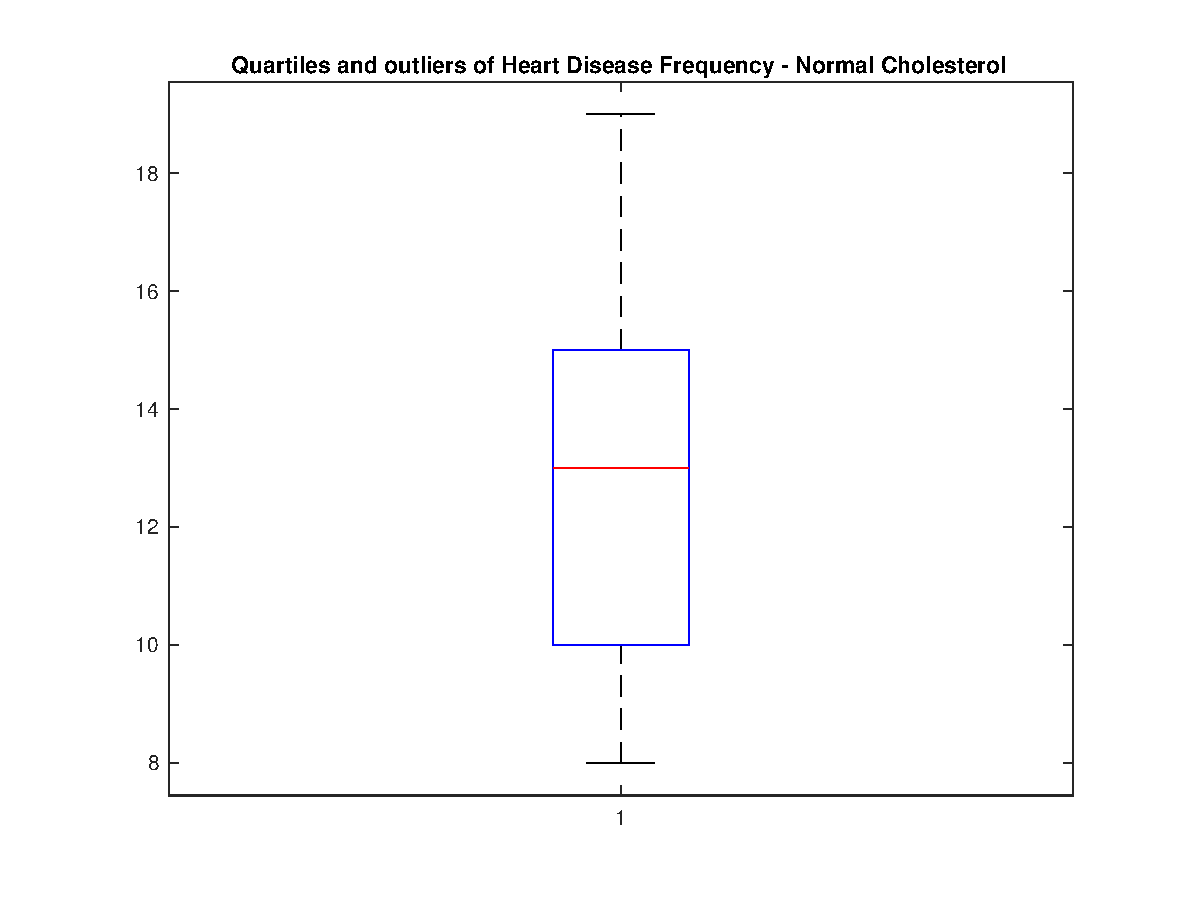
\includegraphics[scale=0.55]{boxplotfinal}
\caption{Box and whisker plot of tularemia infection counts.\label{F:BoxAndWhiskerTularemia}}
\end{figure}
Alternatively, we may also visualize the frequencies of the different outcomes (as well as the central tendency and variability within the data) through the use of a histogram.  Most notably, our histogram (pictured in figure \ref{F:absoluteFrequencies}) clearly shows a mode of 11 and is reasonably suggestive of a unimodal data set.
\begin{figure}
\centering
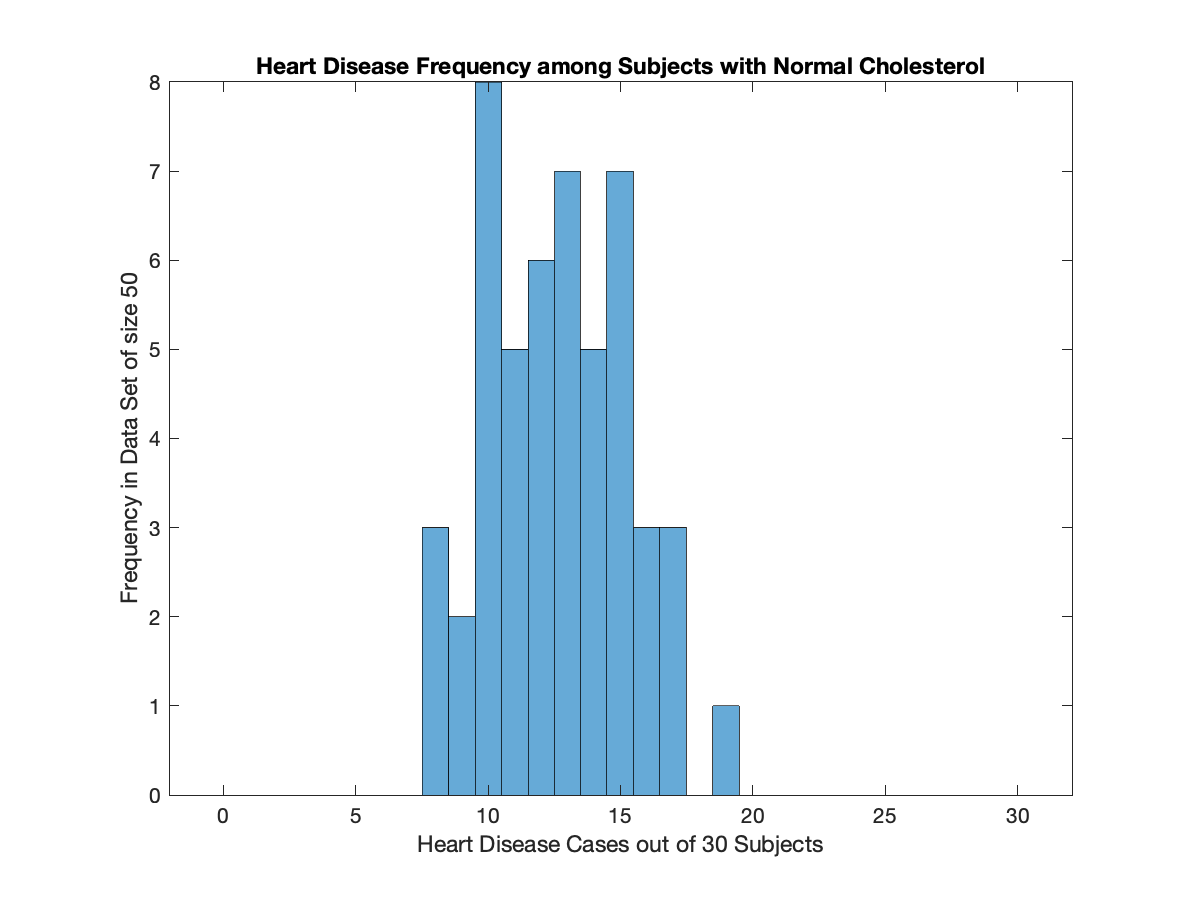
\includegraphics[scale=0.55]{histogramfinal}
\caption{Absolute frequencies of infected rabbit counts within forty samples of thirty rabbits each.\label{F:absoluteFrequencies}}
\end{figure}
In this initial study, we have reported the rudimentary, descriptive statistics of a data set that assesses the occurrence of Tularemia disease in cottontail rabbits throughout the rocky mountain region.  These statistics, include minimum and maximum numbers of diseased rabbits observed in the captured populations, the sample mean and mode, the three quartiles, and the sample variance and standard deviations.  We also provided visual summaries of these statistics and their relationship to our data set with the aid of a box and whisker plot and a histogram.
\section{A Model for Data Collection}
Since, in each habitat, the researchers captured and euthanized thirty rabbits from a larger population, our data collection procedure is an example of sampling without replacement. The size of each sample collected is $n=30$ rabbits.   Since the researchers test each rabbit in the sample for Tularemia and record the number observed, we can understand that these observations are what constitute the outcomes of our data collection procedure.  Therefore, the possible outcomes of our system are the possible observations of anywhere from 0 to 30 infected rabbits in any given sample.  In other words, our sample space is the set $$\Omega=\{x: 0\le x\le 30\},$$  where $x$ represents the number of infected rabbits observed in a sample.  Therefore, this sample space is finite. With a finite sample space, it is often convenient to construct a $\sigma$-algebra for our probability space by forming the power set, or set of all subsets, of the sample space.  Therefore, the $\sigma-$algebra $S$ will consist of the  $2^{31}$ (or roughly two billion) possible subsets of $\Omega$. These make up the measurable events in what will be come a probability space once we devise a way of assigning probabilities to them.

Since we are sampling $n=30$ rabbits without replacement from a population of $N$ rabbits that includes a subcategory of $K$ infected rabbits, and since we are interested in observing the number $x$ of infected rabbits in our sample, it is arguable that our data can be modeled with the hypergeometric distribution
\[
H(N,K,n;x)=\frac{\binom{K}{x}\binom{N-K}{n-x}}{\binom{N}{n}}.
\]
This distribution predicts the probability of observing any value $x$ from our sample space. We may use it to compute the probability of any event $E$ in $S$ by summing the probabilities of each outcome in $E$:
\[
P(E)=\sum_{x\in E} H(N,K,n;x).
\]
As such, the hypergeometric distribution generates the probability measure of the probability space that models our data collection approach. However, in order to make use of this distribution in this way, we will need to be able to measure or estimate the unknown parameters $N$ and $K$.
\section{Derivation of a Theoretical Distribution through Parameter Estimation}
As already stated, in order to model our data collection with the hypergeometric distribution, we will need to estimate the parameters $N$ and $K$. Recall $N$ represents the total population being sampled from and $K$ represents the number of infected rabbits in the total population.  In addition, $n=30$ represents the sample size, and $x$ represents the number of infected rabbits in the sample. Since, we have no idea of the values for $N$ and $K$, we may use the method of moments to estimate both parameters.  However, it is best not to estimate both of these parameters simultaneously.  Therefore, we will first employ a mark and recapture technique to estimate $N$.  Once $N$ is known, we’ll use the tularemia data in order to estimate $K$.
In order to employ mark and recapture, we capture a group of $K_0=100$ rabbits, tag one of their ears, and re-release them into the habitat.  After they’ve had a chance to redistribute themselves, we capture 8 samples of 30 rabbits and count the number of tagged rabbits in each one.  The resulting data set is 
\[
M=\{3, 0, 2, 4, 1, 1, 4, 2\}.
\]
This data ought to be distributed according to a hypergeometric distribution with the unknown total population of $N$, the tagged subcategory of $K=K0=100$, and a sample size of $n=30$.  Therefore, the method of moments tells us to set up the first moment equation 
\[
\bar{x}_M=\mu=n\frac{K_0}{N},
\]
where $\bar{x}_M=2.1250$ is the mean of $M$. This can be rearranged to show that 
\[
N=\frac{n K_0}{\bar{x}_M}\simeq 1412.
\]
Now we return to our original tularemia data set $D_{control}$ in order to estimate $K$. We’ve already computed the sample mean of $D_{control}$ to find $\bar{x}_{control}=11.35$.  Once more, the first moment equation is
\[
\bar{x}_{control}=\mu=n\frac{K}{N}.
\]
When we rearrange this time for $K$, we obtain
\[
K=\frac{\bar{x}_{control} N}{n}\simeq 534.
\]
Therefore, we may try modeling our data set with a hypergeometric distribution using the estimated parameters $N=1412$, $K=534$, and $n=30$.  If we plot the graph of the probability mass function for this theoretical distribution on the same axes as our normalized empirical distribution (see figure \ref{F:graphicalAssessement}), we can see that agreement between the two appears to be qualitatively good.  This suggests that we are on the right track with this choice of model.
\begin{figure}
\centering
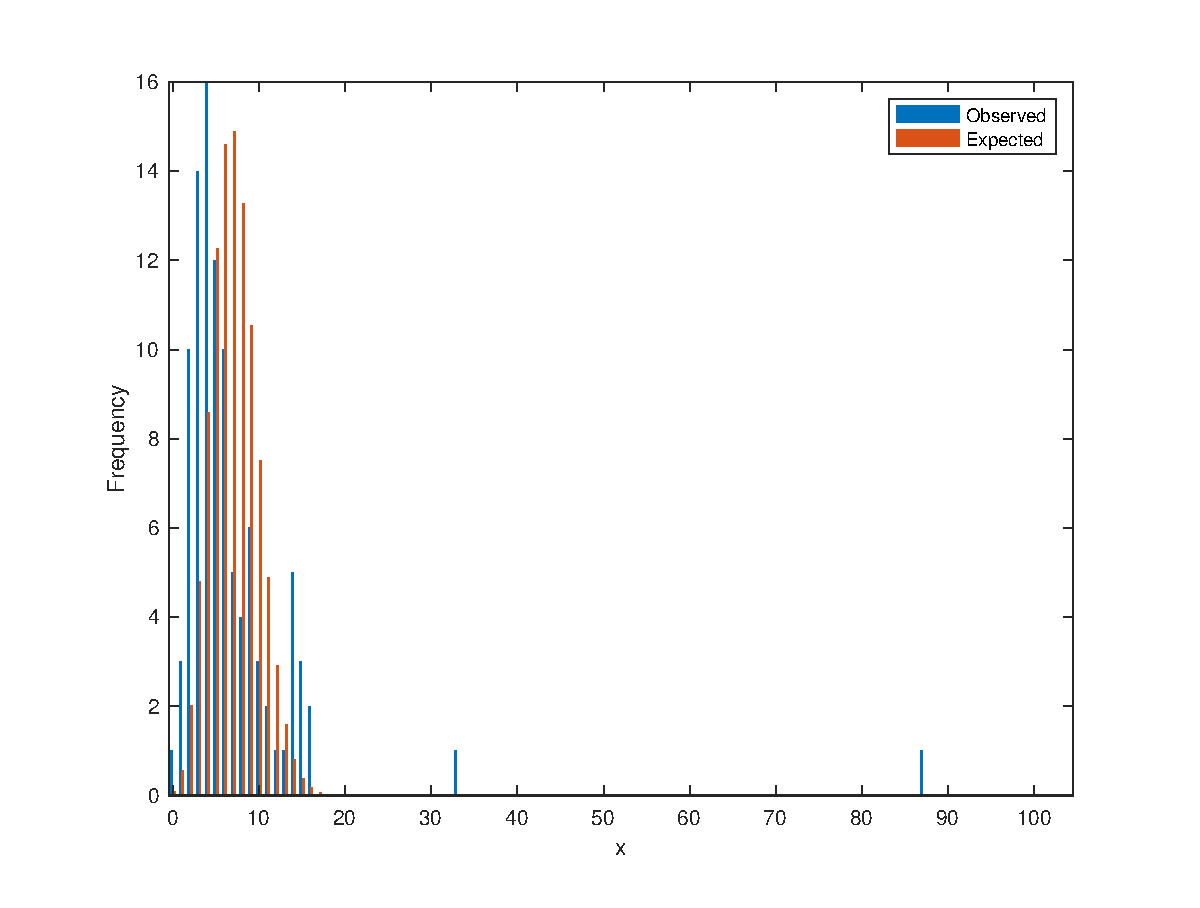
\includegraphics[scale=0.55]{histvalidationfinal}
\caption{
Comparison between empirical relative frequencies and theoretical, hypergeometric model.\label{F:graphicalAssessement}}
\end{figure}
Moreover, we can also compute the theoretical values of mean, variance, skewness, and kurtosis for this calibration of the hypergeometric distribution and compare them to the values we have already computed for our data set. This comparison is summarized in Table \ref{Tbl:quantitativeAssessment}.
\begin{table}
\begin{tabular}{lrrrr}
\toprule
			&	{\bf Mean}	&	{\bf Variance}	&	{\bf Skewness}	&	{\bf Kurtosis}\\\midrule
{\sl Theoretical}	&	11.3500	&	7.2775		&	0.41339		&	2.8657\\ 
{\sl Empirical}		&	11.3460	&	6.9099		&	0.088868		&	2.9436\\
\bottomrule
\end{tabular}
 \caption{Quantitative comparison of the theoretical shape parameters of the model distribution to the empirical shape parameters of the data set.\label{Tbl:quantitativeAssessment}}
\end{table}
Again, agreement between the empirical and theoretical shape parameter values is somewhat close, so this further corroborates the idea that our choice of the hypergeometric distribution as a theoretical model for our data. 

Another fit assessment we can perform is to construct a quantile-quantile plot, or QQ plot, in which we plot the quantiles of each data point in $D_{control}$ against the theoretical quantiles of the hypergeometric distribution. When the distribution fits the data well, the QQ plot should show a linear relationship between the empirical and theoretical quantiles. Our QQ plot is displayed in figure \ref{F:qqplot}, and it is evident that such a linear relationship exists. This is yet another indication that our model fits our data well.
\begin{figure}
\centering
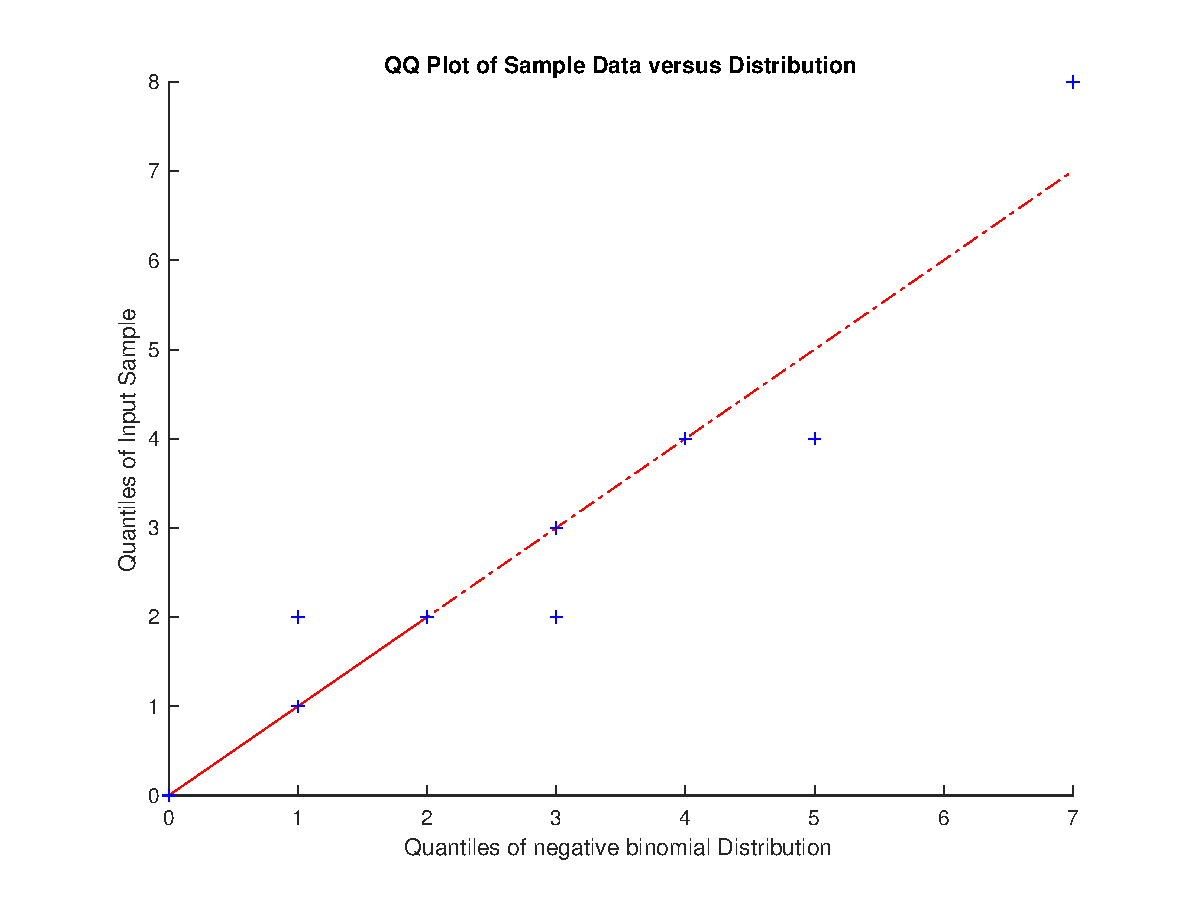
\includegraphics[scale=0.55]{qqplotfinal}
\caption{
Quantile-quantile plot expressing the relationship between the observed quantiles of each point in $D_{control}$ and the theoretical quantiles of the hypergeometric distribution. The relationship appears to be linear, which indicates a good fit..\label{F:qqplot}}
\end{figure}

Finally, we can be more quantitative still in comparing the data to the hypergeometric model by performing a goodness of fit test.  To do so, we pool the possible values from the sample space into bins that ensure there is an expected frequency ($E$) (predicted by the hypergeometric distribution) of at least 5 observations per bin.  Then, we compare these predictions to the actual frequencies observed ($O$) in these bins in our data set.  This information is summarized in the Table \ref{Tbl:chi2}.

\begin{table}
{\footnotesize
\begin{tabular}{lccccc}
\toprule
\multirow{2}{*}{Frequencies} & \multicolumn{5}{c}{Bins}\\	
	& $0\le x\le 9$ &	$9<x\le 10$ & 	$10<x\le 11$ & 	$11<x\le 12$ &	$12<x\le 30$\\
	\midrule
Observed& 11& 4& 7& 6& 12\\
Expected & 9.7590& 5.4116& 6.0021& 5.7794& 13.0479\\
\bottomrule
\end{tabular}}
\caption{Expected and observed frequencies of tularemia infection counts in samples of size $n=30$ taken from populations of cottontail rabbits.\label{Tbl:chi2}}
\end{table}

From this data, we may compute the $\chi^2$ test statistic.
$$\chi^2=\sum\frac{(E(x)-O(x))^2}{E(x)}=0.7845$$
In order to compare this to an appropriate chi squared distribution, we need to determine the number of degrees of freedom for the comparison of our frequencies.  We have organized our frequencies into 6 bins.  However, in order to compute the expected frequencies, we used the hypergeometric distribution with estimated values for both $N$ and $K$.  We also are assigning 6 frequency counts out of a total of 40 observations to six bins. This means that there are $\nu$=5 bins-2 estimated parameters-1 dependency=2 degrees of freedom. According to the $\chi^2$ distribution with $\nu=2$ degrees of freedom, the probability of observing a $\chi^2$ statistic at least as high as ours is
$$P(\chi^2\ge 0.7845;\nu=2)=0.6755.$$
This value is not small enough to reject the null hypothesis that states our model fits our control data well, so we conclude that the expected frequencies predicted by the hypergeometric distribution are an adequate fit to the data we've collected.
\section{Hypothesis Testing: Impacts of Climate upon Tularemia Prevalence}
For quite some time, it has been suspected that Tularemia outbreaks can be mitigated in rabbit populations if longer, colder winters occur (especially if the additional cold weather occurs earlier in the year, towards autumn) .  The researchers had four additional rabbit populations available to them that were comparable to the others in the study.  However, these populations experienced a particularly long and cold winter that the others did not.  Therefore, before sampling these populations, the researchers devised a null hypothesis:
\begin{description}
\item[$H_0$ (null hypothesis)] We will not observe significantly different numbers of rabbits infected with Tularemia in the cold climate samples than we observe in the other samples. 
\end{description}
With this hypotheses in place, we set out to determine the significance of each point in our experimental data set:  They found that these samples contained only 
\[D_{experimental}=\{4, 1, 6, 8, 6, 5, 4, 3\}\].
These values appear to be different from the data collected from the original 40 populations, but the question of whether this difference is significant still remains.  To answer it, we use our theoretical, hypergeometric distribution (with parameters $N=1412$, $K=534$, and $n=30$) to compute P-values for our eight experimental observations. First we test for a significant increase of each point in $D_{experimental}$ compared to what is expected from $D_{contol}$ by computing $P$ values for each point in $D_{experimental}$:
\[
P_{H,increase}=\sum_{x=x_0}^n H(N,K,n;x).
\]  These are:
\[
P_{H,increase}=\{0.9994, 1.0000, 0.9899, 0.9315, 0.9899, 0.9971, 0.9994, 0.9999\}.
\]
None of these are high enough to reject $H_0$ on the basis that the experimental data is surprisingly high.

Next, we test for a significant decrease of each point in $D_{experimental}$ compared to what is expected from $D_{contol}$ by computing $P$ values for each point in $D_{experimental}$:
\[
P_{H,decrese}=\sum_{x=0}^{x=x_0}H(N,K,n;x).
\]  These are:
\[
P_{H,decrease}=\{0.0029, 0.0000, 0.0289, 0.1387, 0.0289, 0.0101, 0.0029, 0.0006\}.
\]
All but one of these is low enough (well below 5\%) to warrant rejecting the null hypothesis on the basis that the experimental data is surprisingly low. This is certainly evidence for a correlative relationship between habitat climate and tularemia infection rates. Whether a causal relationship exists would require further study.

We could also take some alternative approaches by considering our eight experimental data points, 
\[D_{experimental}=\{4, 1, 6, 8, 6, 5, 4, 3\}\]
to be a sample of observations. From this point of view, we can consider whether the mean of this sample
$$\bar{x}_e=4.6250$$
is significantly different from the theoretical mean of the hypergeometric distribution 
$$\mu=\frac{n K}{N}=11.35$$
by performing a one sample t-test. The sample standard deviation of the experimental sample is $$s=2.1339.$$ Therefore, the t statistic is given by
$$T=\frac{\bar{x}-\mu}{s/\sqrt{8}}=-8.9079$$
We can set a new null hypothesis:
\begin{description}
\item[$H_0$ (null hypothesis)] There is no significant difference between the mean number of rabbits infected with Tularemia in the cold climate habitat in comparison and the theoretical mean number of infected rabbits in the control climates. 
\end{description}
The one sample t-test returns a p value of $4.5605\times 10^{-5}$ and predicts a 95\% confidence interval of $2.8410\le \bar{x}\le 6.409$ for the location of the true mean of the population the experimental data set was sampled from. 

Alternatively, we could also employ the two sample t-test for determining if there is a significant difference between the means of the experimental and control data sets. There are at least three advantages of doing so. First, this approach does not require us to assume any knowledge of the theoretical mean (or the corresponding theoretical distribution) of the population the control data set was sampled from. We are pretty well justified in modeling the control data set with the hypergeometric distribution, but this won't always be the case in other experiments. Second, the two sample t-test is a little more conservative than the one sample test, so if we are able to establish significance with it, then we are doing so in a more grounded way. Finally, we may relax any assumptions about the equality between the variances of the  experimental and control populations\footnote{If we were truly concerned about determining if there is a significant difference between the variances of the experimental and control populations, we could employ either the $\chi^2$ test for comparing the sample variance of the experimental data set to the theoretical variance of the control population or the F test for comparing the variances of the experimental and control data sets. The p values for these tests repectively are 0.5859 and 0.5119. In both cases, this represents a lack of evidence for a significant difference between the variances.}. In any case, the null hypothesis for the two sample t-test is
\begin{description}
\item[$H_0$ (null hypothesis)] There is no significant difference between the means of the experimental and control data sets.
\end{description}
The two sample t-test returns a p-value of $5.0108\times 10^{-6}$. It also returns a 95\% confidence interval for the location of the difference between the true means of the experimental and control populations: $-8.6173\le \bar{x_E}-\bar{x_C} \le -4.8326$.
As we saw with the discrete tests using the hypergeometric distribution, this result signifies that the data supports rejecting the null hypothesis on the basis that the mean of the experimental data appears surprisingly lower than what is expected of the control data. 
\section{Conclusion}
In this initial study, we were interested in determining whether we could find evidence consistent with the hypothesis that there is a difference in tularemia frequency when examining rabbit populations taken from populations in colder climates vs. more moderate climates. We have collected (without replacement) samples of rabbits from several similar populations that live in moderate climates, tested them for tularemia, and recorded the numbers who tested positive. In this way we built a control data set that we believed could be modeled with a hypergeometric distribution. We built an experimental data set applying the same sampling methodology to several populations living in colder climates. We then used the method of moments in order to estimate the unknown parameters N and K for the hypergeometric distribution so that we could use it as a model for our control data set.  We validated this model using both qualitative and quantitative measures. Finally, we performed several complementary hypothesis tests to determine if our experimental data set could be viewed as evidence for rejecting the null hypothesis that there is no significant difference between the counts of infected rabbits (or their means) and the expected levels established by the control data. We found statistically significant results that suggest there are significantly lower numbers of infected rabbits in colder environments.
\end{document}
